\documentclass{article}
\newcounter{minitocdepth}
\newcounter{chapter}
\newcommand{\chaptername}{}
\usepackage{iesbbook}
\newcommand{\vs}{\vspace{0cm}}
\geometry{a4paper,total={170mm,257mm},left=30mm,right=23mm,top=15mm,bottom=15mm}
\begin{document}
 
\begin{center}
\underline{\textbf{\large PROPORCIONALITAT COMPOSTA}}

\end{center}
	
	\begin{mylist}
		\item El lloguer de 2 cotxes durant 9
		dies costa 675 \euro{}. Quant costarà llogar 5 cotxes durant 7 dies?
		\begin{example}
			
			\begin{minipage}{0.6\textwidth}
					Plantejam el problema amb les tres magnituds que apareixen ``cotxes", ``Dies'' i ``Preu". 
				Ara ens fixam quina és la relació entre la magnitud que ens demanen ``Preu" amb cadascuna de les altres.
				Com més cotxes, major el preu (Directa). Com més dies lloguem, major el preu (Directa).
				  
			\end{minipage}
			\begin{minipage}{0.4\textwidth}
				\centering
					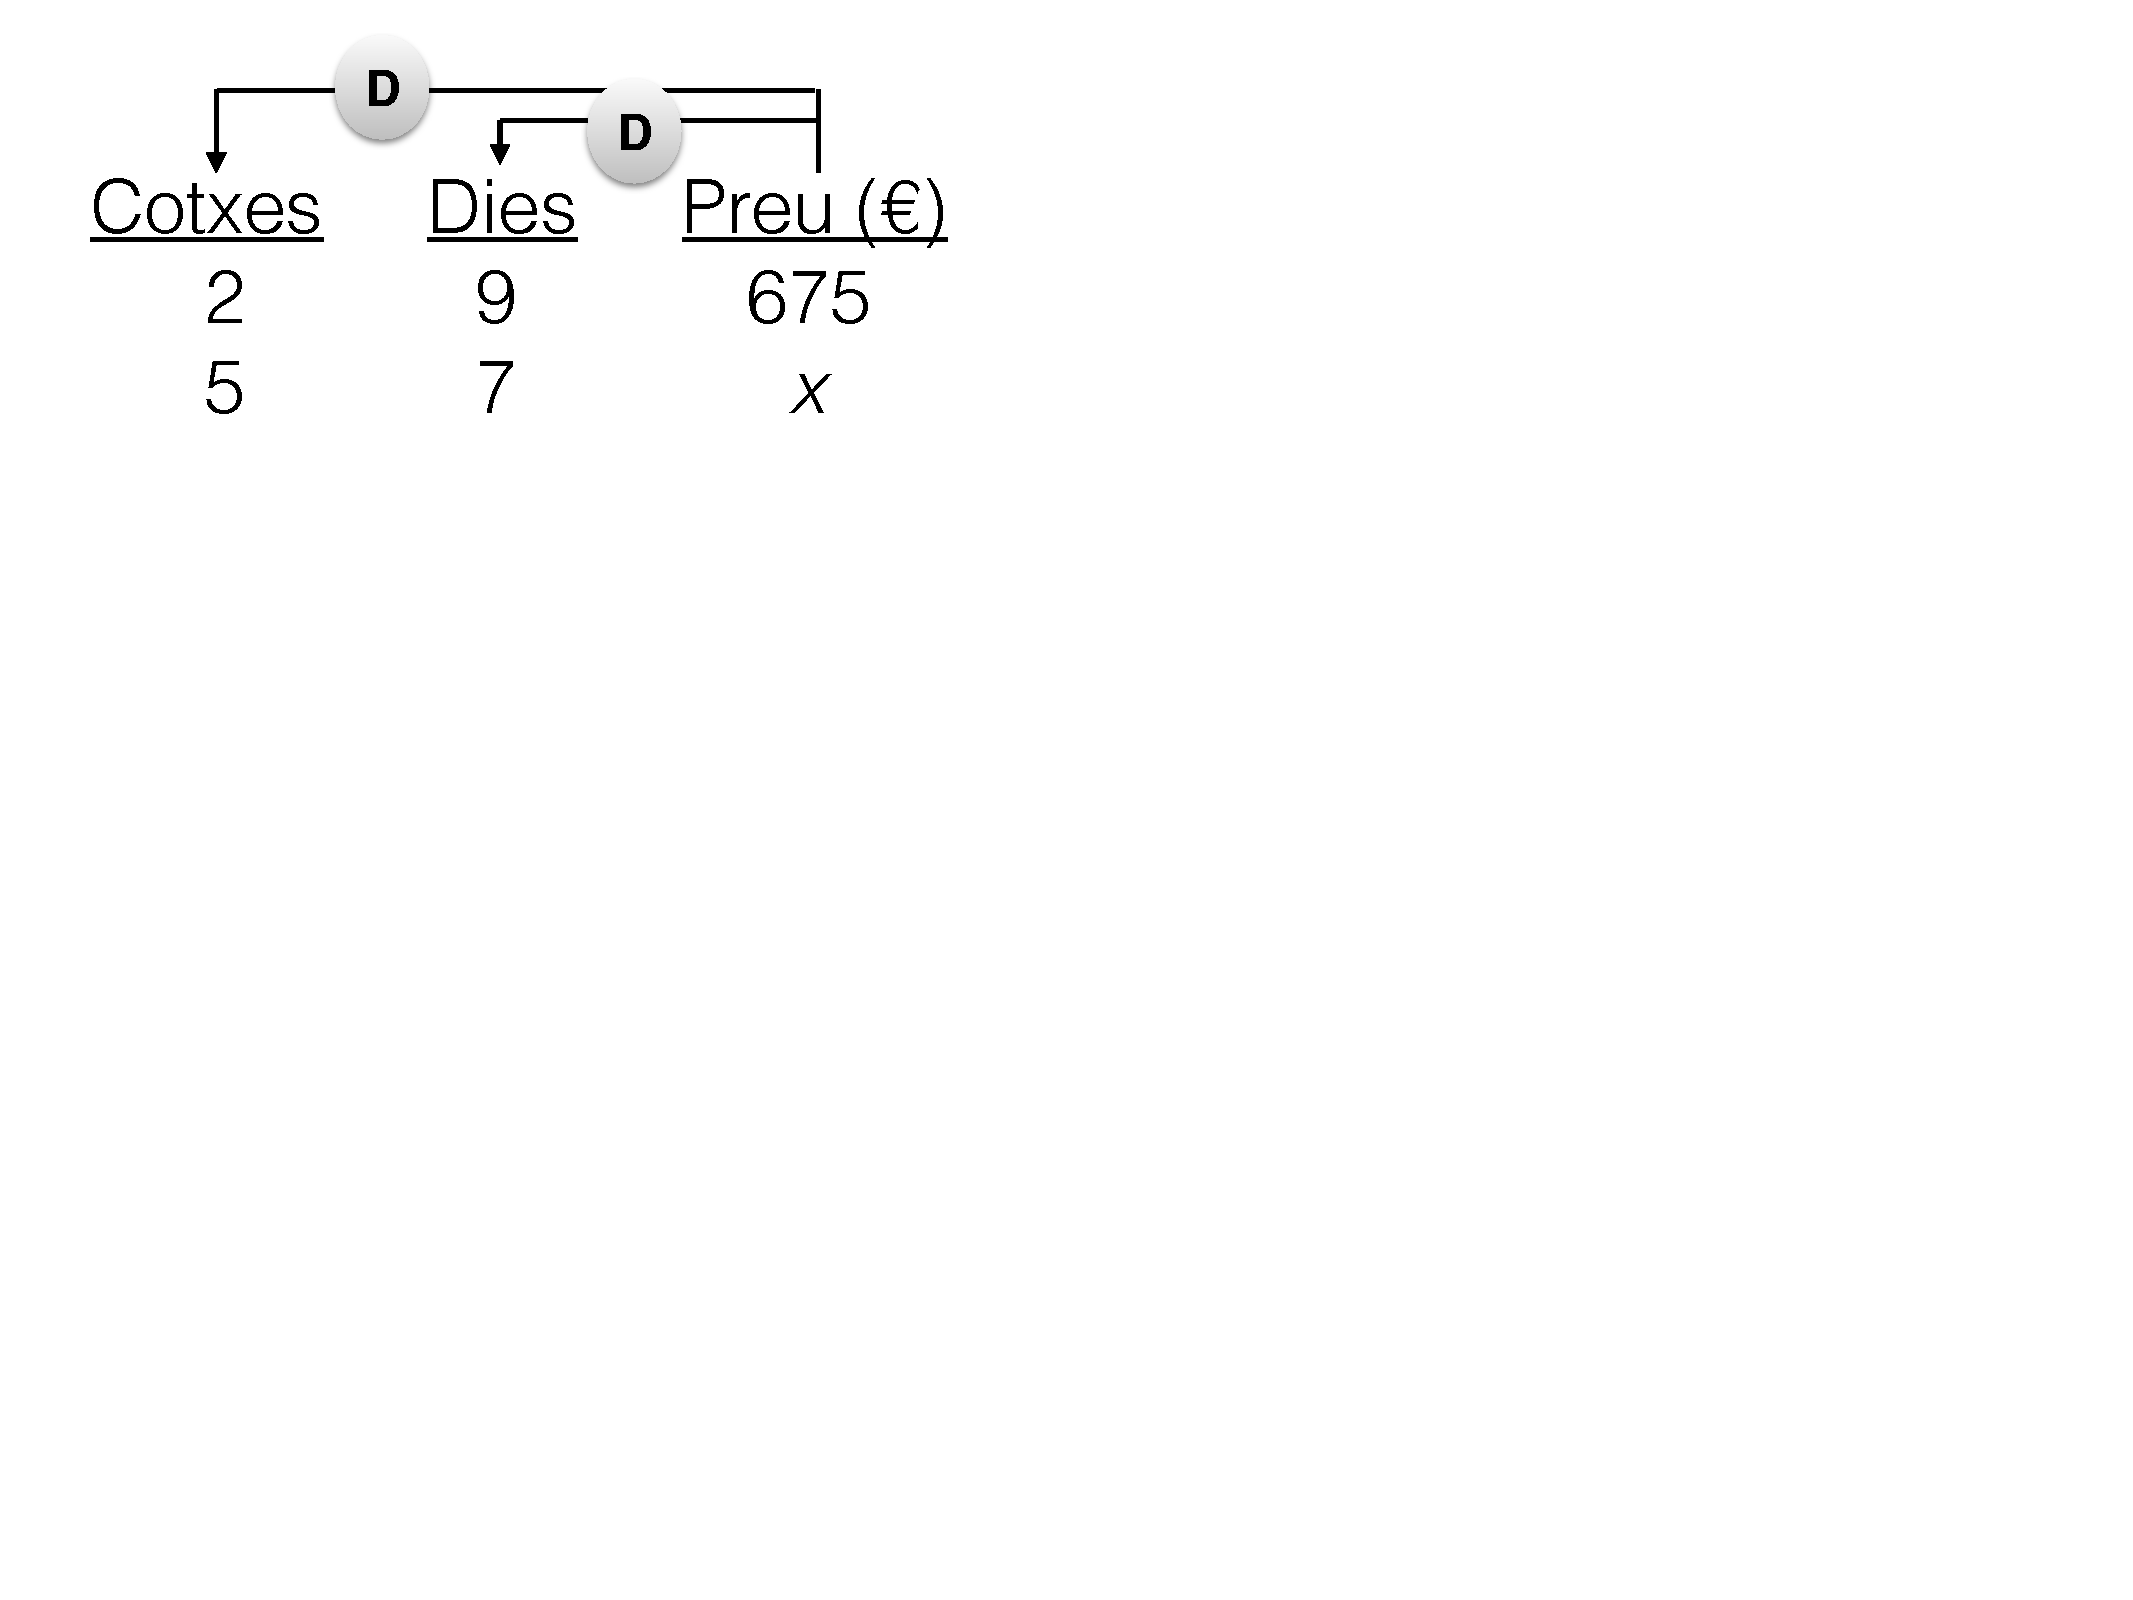
\includegraphics[width=5cm]{img7/proporcionalitat}
			\end{minipage}
		
		\[ \frac{675}{x} = \frac{2}{5} \cdot \frac{9}{7} \quad \rightarrow \quad \text{Aïllam la }x \quad x=\frac{675\cdot 5 \cdot 7}{2\cdot 9}= 1312,50 \text{ \euro}  \]
		\end{example}
		\vs\vs\vs
		\item Tres treballadors recullen 300 kg de raïm en 2 dies. Quant tardaran 4 treballadors a recollir 500 kg del mateix raïm?
			\begin{example}
			
			\begin{minipage}{0.6\textwidth}
				Plantejam el problema amb les tres magnituds que apareixen ``Treballadors", ``Kg raïm'' i ``Dies". 
				Ara ens fixam quina és la relació entre la magnitud que ens demanen ``Dies" amb cadascuna de les altres.
				Com més treballadors, menys dies (Inversa). Com més Kg, més dies (Directa).
				
			\end{minipage}
			\begin{minipage}{0.4\textwidth}
				\centering
				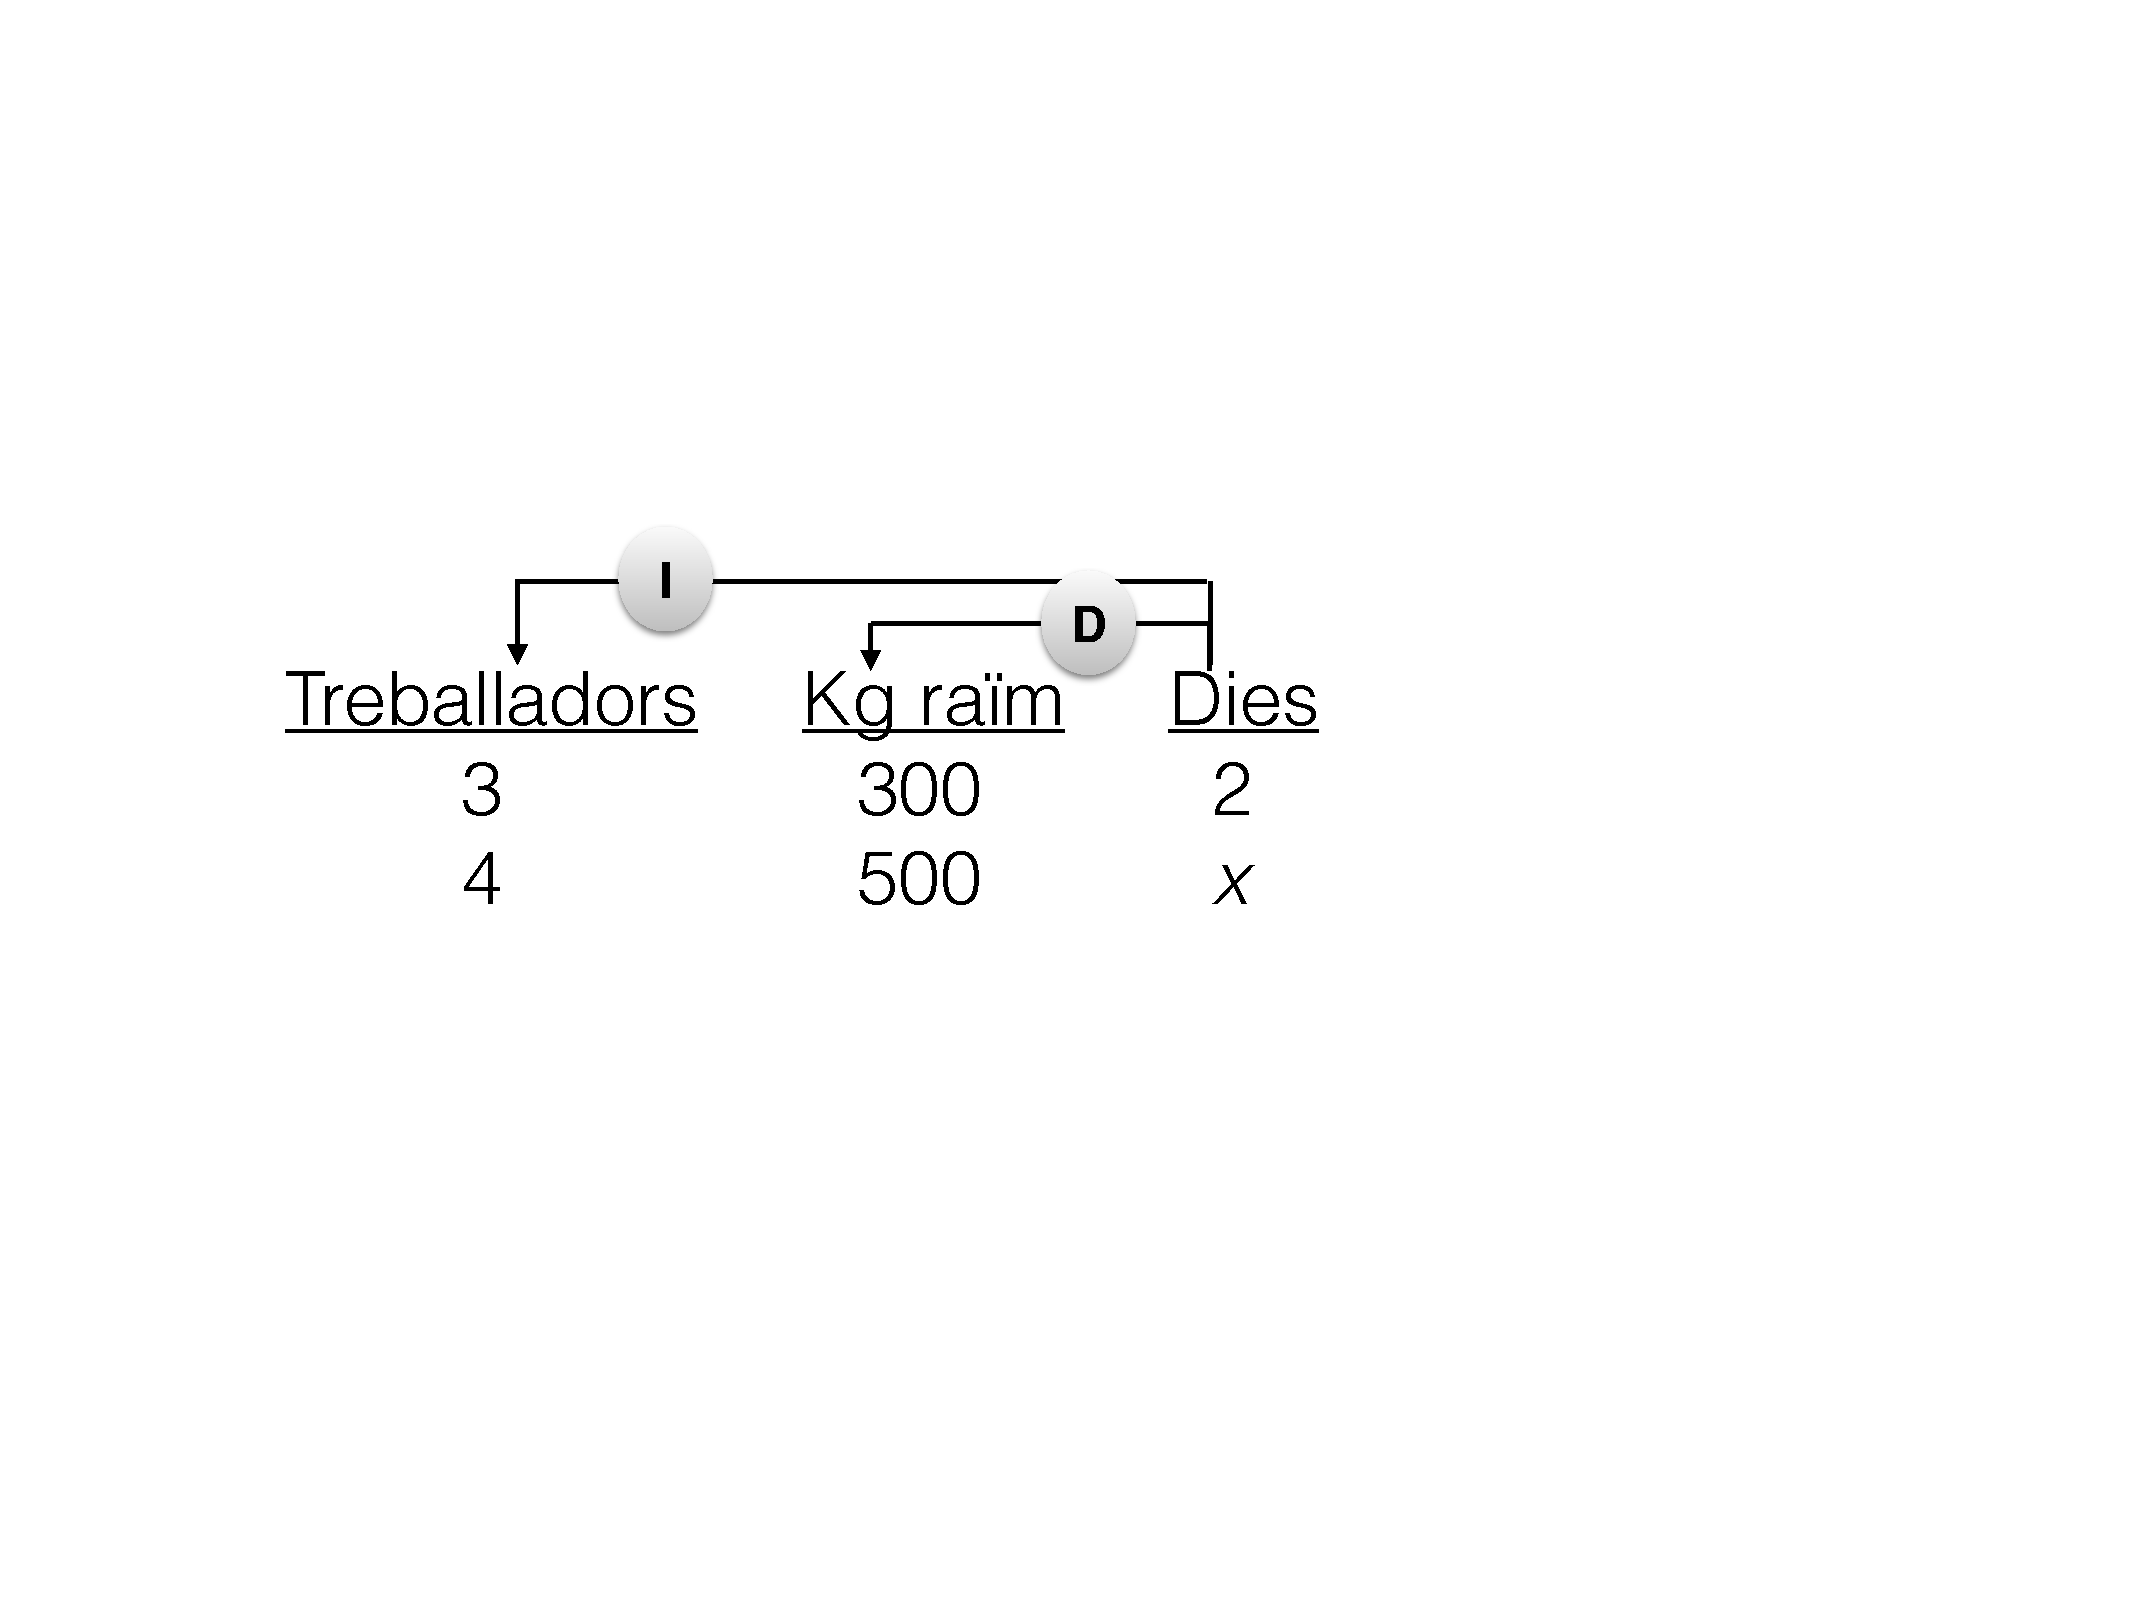
\includegraphics[width=5cm]{img7/proporcionalitat2}
			\end{minipage}
			
			\[ \frac{2}{x} = \boxed{ \frac{4}{3} } \cdot \frac{300}{500} \quad \rightarrow \quad \text{Aïllam la }x \quad x=\frac{2\cdot 3 \cdot 500}{4\cdot 300}= 2,5 \text{ dies}  \]
			
		\end{example}
	\vs\vs\vs
		\item
		Una barra de metall de 10 m de llarg i 2 cm\textsuperscript{2} de
		secció pesa 8,45 kg. Quant pesarà una barra del mateix material de 5 m
		de llarg i 7 cm\textsuperscript{2} de secció.	\vs
		\item
		Sabem que dues màquines funcionant 6 hores diàries consumeixen 1500
		kW/h al dia. Durant quantes hores al dia haurien de treballar 5
		màquines si volem que el consum no superi els 5000 kW/h?	\vs
		\item
		Si 12 excavadores fent feina 10 dies han remogut 360
		m\textsuperscript{3} de terra, quants de dies tardaran 8 excavadores a
		remoure 620 m\textsuperscript{3} de terra?	\vs
		\item
		Un total de 18 operaris, fent feina 6 hores diàries, han tardat 6 dies
		a instal·lat 300 m de cable. Quantes hores diàries han de fer feina 24
		operaris durant 14 dies per instal·lar 700 m de cable?	\vs
		\item
		L'any passat teníem un pressupost per al menjador de l'escola de
		34.000 \euro{} mensuals per alimentar 262 alumnes. Si aquest any hi ha
		22 alumnes més però el pressupost només ha augmentat en 1.200 \euro{}
		mensuals, durant quants de dies podrem oferir el servei de menjador?	\vs
		\item
		Sabem que 9 ordinadors encesos durant 10 hores diàries produeixen una
		despesa de 2340 \euro{} anuals. Quina seria la despesa si
		s'encenguessin 6 ordinadors més durant una hora menys al dia?	\vs
		\item
		Una família de sis membres consumeix 2 kg de pa cada 5 dies. Quants de
		dies els durarien 3 kg de pa a una família de 8 membres amb un consum
		similar?	\vs
		\item
		Amb quatre fotocopiadores es fan 30.000 còpies fent feina 3 hores
		diàries. Quantes còpies es podrien fer amb 5 fotocopiadores fent feina
		durant 2 hores diàries?	\vs
	\end{mylist}
\end{document}